\section{Problem Formulation and Benchmark}

\subsection{Row-level Prediction Task}

Let \(t\) denote a tissue and \(m\) an MHC-I restriction. We define the set of observed prediction tasks as
\[
\mathcal{T}=\{\tau=(t,m)\}.
\]
Each benchmark row is represented by
\[
x_i=(p_i,\tau_i), \qquad y_i\in\{0,1\},
\]
where \(p_i\) is a nine-residue peptide and \(\tau_i\) is a tissue--MHC task. A positive label, \(y_i=1\), indicates that the peptide has positive ligand evidence in the target tissue--MHC context. A pseudo-negative label, \(y_i=0\), indicates that the peptide has positive evidence under the same MHC restriction and parent protein in at least one other tissue, but is not reported for the target tissue--MHC task. Thus, a pseudo-negative is an absence-of-evidence construction rather than an experimentally verified non-presented peptide.

Given \((p,\tau)\), a model parameterized by \(\theta\) produces
\[
s_{\theta}(p,\tau)\in\mathbb{R},
\]
with larger values indicating stronger predicted presentation-evidence preference within task \(\tau\). Training is performed as row-level binary classification. The paired structure determines how examples are constructed, controlled, split, and evaluated, but the primary models do not directly optimize a pair-ranking loss. Because prediction heads are task specific, the benchmark evaluates tasks represented during training; it does not by itself assess unseen tissues or unseen MHC restrictions.

\subsection{Matched Pair Structure}

Each pair \(j\) contains exactly one positive peptide \(p_j^{+}\) and one pseudo-negative peptide \(p_j^{-}\). The two rows share the same target tissue, MHC restriction, and parent UniProt protein:
\[
t_j^{+}=t_j^{-}, \qquad
m_j^{+}=m_j^{-}, \qquad
u_j^{+}=u_j^{-}.
\]
Matching removes the nominal presenting molecule as a between-label difference and holds source-protein identity constant. The model must therefore distinguish two peptides from the same protein using task-conditioned evidence. Antigen processing, tissue composition, study design, detection sensitivity, and annotation completeness remain uncontrolled.

The primary evaluation aggregates AUROC and AUPRC at the task level so that large tasks do not dominate the benchmark. We additionally define paired concordance as
\[
\mathrm{PairAcc}
=
\frac{1}{N}
\sum_{j=1}^{N}
\mathbf{1}
\left[
s_{\theta}(p_j^{+},\tau_j)
>
s_{\theta}(p_j^{-},\tau_j)
\right],
\]
where \(N\) is the number of held-out pairs. PairAcc directly measures whether the positive member of each matched pair receives the higher score. It complements rather than replaces task-macro AUROC, because the latter evaluates ordering across all positive and pseudo-negative rows within each task.

\subsection{Evidence Selection and Normalization}

The human and mouse benchmarks are derived from the IEDB full MHC ligand export downloaded on July 4, 2026 \cite{vita2025iedb}. Human and mouse records are processed separately under the same inclusion logic. A retained record must satisfy all of the following criteria:

\begin{itemize}
    \item a qualitative measurement whose normalized text begins with \emph{positive};
    \item MHC class I restriction, with both peptide source and host matching Homo sapiens for the human benchmark or Mus musculus for the mouse benchmark;
    \item a human restriction matching the four-digit HLA pattern \texttt{HLA-...*dd:dd} (the extractor also accepts the equivalent colon-free four-digit form) or a mouse restriction beginning with \texttt{H2-};
    \item a parent UniProt accession extracted from the IEDB molecule-parent IRI;
    \item a linear, unmodified peptide containing only the 20 standard amino acids;
    \item a peptide length of exactly nine residues; and
    \item deduplication before pairing by the exact peptide, restriction, tissue, and parent/source-protein annotation fields.
\end{itemize}

Source-tissue values are stripped of surrounding whitespace and retained as exact IEDB task labels; distinct nonempty tissue strings are not merged after extraction. Empty or \texttt{NA}-like task fields are removed before benchmark filtering, which excludes 857 otherwise eligible human pairs, and pair-consistency checks require both rows to have the same nonempty tissue and restriction. Retained HLA and H2 strings are used directly as task identifiers after the pattern checks above. Records without a parent UniProt accession are excluded because parent-protein matching is a defining control of the benchmark. Restricting the study to unmodified canonical 9-mer MHC-I peptides provides a consistent sequence space, but excludes variable-length ligands, post-translationally modified peptides, and MHC-II presentation.

\subsection{Pair Construction}

Pairs are generated independently within each target tissue--MHC task with random seed 20260704. The construction procedure is:

\begin{enumerate}
    \item Group all eligible ligand records by MHC restriction \(m\) and parent UniProt protein \(u\).
    \item For each target combination \((t,m,u)\), collect peptides with positive evidence in tissue \(t\).
    \item From other tissues represented in the same \((m,u)\) group, collect candidate pseudo-negative peptides.
    \item Exclude every candidate that has any positive report in the target tissue--MHC task \((t,m)\).
    \item Within each target task and label, use each peptide at most once. For a given \((t,m,u)\) group, set the number of pairs to the smaller of the eligible positive and pseudo-negative counts and sample both sets without replacement.
    \item Randomly permute the selected pseudo-negatives and zip them one-to-one with the selected positives.
    \item Assign a persistent pair identifier, preserve the reported-tissue and protein annotations, and audit that every identifier has exactly one row per label, matched tissue, restriction, and parent UniProt, with no pseudo-negative reported in the target task.
\end{enumerate}

This procedure yields an intentionally balanced row-level dataset because every pair contributes one row of each label. Consequently, benchmark AUPRC values must not be interpreted as performance under the prevalence encountered in an unfiltered tissue sample. The labels represent relative evidence within the constructed comparison set, not calibrated absolute presentation probabilities.

\begin{figure}[tbp]
\centering
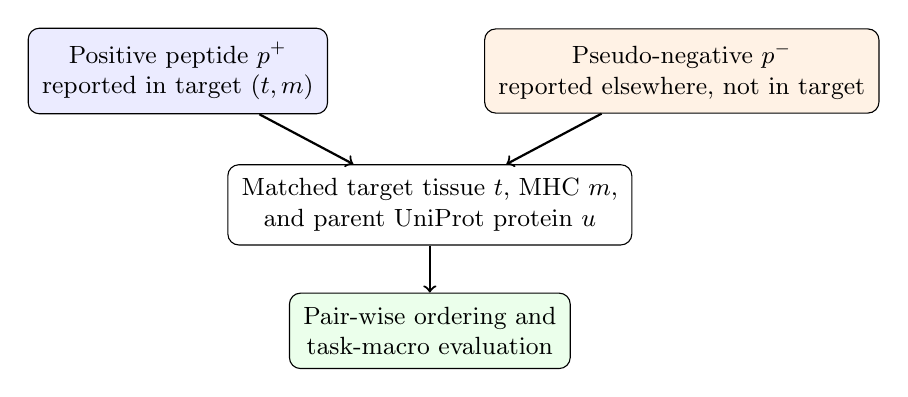
\begin{tikzpicture}[
    node distance=0.7cm,
    box/.style={draw,rounded corners,align=center,inner sep=5pt,font=\small},
    arr/.style={->,thick}
]
\node[box,fill=blue!8] (pos) at (-3.2,0) {Positive peptide \(p^{+}\)\\reported in target \((t,m)\)};
\node[box,fill=orange!10] (neg) at (3.2,0) {Pseudo-negative \(p^{-}\)\\reported elsewhere, not in target};
\node[box] (match) at (0,-1.7) {Matched target tissue \(t\), MHC \(m\),\\and parent UniProt protein \(u\)};
\node[box,fill=green!8] (eval) at (0,-3.3) {Pair-wise ordering and\\task-macro evaluation};
\draw[arr] (pos) -- (match);
\draw[arr] (neg) -- (match);
\draw[arr] (match) -- (eval);
\end{tikzpicture}
\caption{Matched-pair construction. Both rows share the target tissue, MHC restriction, and parent protein; the pseudo-negative has positive evidence elsewhere but no report in the target task.}
\label{fig:pair-construction}
\end{figure}

\subsection{Human Benchmark}

The primary human benchmark retains tissue--HLA tasks with strictly more than 200 eligible pairs. Within each retained task, exactly 100 pair identifiers are sampled without replacement for the standard fixed test and all remaining pairs form the training partition, using split seed 20260704. Its standard pair-disjoint split contains the statistics summarized below.

\begin{table}[tbp]
\centering
\caption{Human standard pair-disjoint benchmark statistics.}
\label{tab:human-benchmark-stats}
\small
\begin{tabular}{lr}
\toprule
Property & Value \\
\midrule
Tissue--HLA tasks & 157 \\
Tissues & 25 \\
HLA alleles & 35 \\
Training pairs & 73,798 \\
Test pairs & 15,700 \\
Training rows & 147,596 \\
Test rows & 31,400 \\
Test pairs per task & 100 \\
\bottomrule
\end{tabular}
\end{table}

The 157-task inventory is summarized in Table~\ref{tab:human-benchmark-stats}. It forms an incomplete and long-tailed tissue-by-HLA coverage matrix rather than a full Cartesian product. Task-wise evaluation is therefore essential: a pooled metric would overweight common tissue--HLA combinations and could conceal weak performance on sparse tasks. The standard benchmark holds out pair identifiers, but a peptide or parent protein may still occur in a different task on both sides of the split. We accordingly treat this protocol as a primary closed-task benchmark rather than evidence of strict entity-level generalization.

For peptide-disjoint evaluation, the complete 73,798-pair human training pool from the standard benchmark---excluding the separate 15,700-pair fixed test---is considered as a single pool. Pairs sharing either peptide are joined through connected components before fold assignment. This produces 17,036 components, including 10,923 multi-pair components; the largest component contains 755 pairs. Deterministic task-stratified assignment distributes complete components across three folds. Each held-out fold contains 24,598--24,600 pairs, each fitting set contains 49,198--49,200 pairs, all 157 tasks remain represented, and both pair and peptide overlap between fitting and held-out data are zero.

\subsection{Mouse Benchmark}

The mouse benchmark is constructed with the same tissue-conditioned, MHC- and parent-protein-matched task definition, using H2 restrictions in place of HLA alleles. Tissue--H2 tasks must contain strictly more than 200 eligible pairs; exactly 100 pair identifiers per retained task are sampled without replacement for the standard fixed test with split seed 20260704, and the remainder form the training partition.

\begin{table}[tbp]
\centering
\caption{Mouse standard pair-disjoint benchmark statistics.}
\label{tab:mouse-benchmark-stats}
\small
\begin{tabular}{lr}
\toprule
Property & Value \\
\midrule
Tissue--H2 tasks & 24 \\
Tissues & 13 \\
H2 restrictions & 4 \\
Training pairs & 6,766 \\
Fixed-test pairs & 2,400 \\
Training rows & 13,532 \\
Fixed-test rows & 4,800 \\
\bottomrule
\end{tabular}
\end{table}

The mouse inventory is summarized in Table~\ref{tab:mouse-benchmark-stats}. The standard mouse evaluation uses a frozen internal pair-disjoint fixed test. Its pair-identifier overlap with training data is zero, but entity overlap remains substantial: 2,453 of 3,011 unique test peptides (81.47\%) and 967 of 1,088 unique test parent proteins (88.88\%) also occur in training. Measured by test rows, the corresponding overlap rates are 84.31\% and 93.04\%. This audit limits the standard fixed test to internal closed-task confirmation and rules out interpreting it as unseen-peptide, unseen-protein, or independent external validation.

The mouse peptide-disjoint protocol applies the same connected-component construction to all 6,766 pairs. Complete components are assigned to three folds while maintaining all 24 tasks in every held-out partition. Pair and peptide overlap are both zero; the largest component contains 50 pairs, and the number of held-out pairs per task ranges from 41 to 157, with 82--314 fitting pairs per task. These counts show that strict peptide separation is feasible without deleting overlapping pairs after an initial random split.

\subsection{Evaluation Splits and Leakage Audits}

We distinguish three evaluation settings throughout the paper. Here, out-of-fold (OOF) prediction means that every reported row is predicted by a model fitted without the fold containing that row. First, the standard pair-disjoint fixed-test or OOF evaluations provide the primary closed-task benchmark results: a pair identifier cannot cross the fitting/held-out boundary, but either peptide may have appeared in another pair or task. Second, a matched standard pair-disjoint OOF control is generated from the same complete pair pool as the strict evaluation, with fold number, task coverage, and task-wise held-out sizes matched as closely as possible. This matched control is the appropriate reference for isolating the effect of peptide separation. Third, connected-component peptide-disjoint OOF evaluation prevents every peptide sequence from appearing in the fitting partition of any task when it is held out. It therefore measures globally unseen-peptide performance for previously represented tissue--MHC tasks, not merely a peptide unseen in one specific task and not an unseen-task setting.

For every split, pairs rather than individual rows are the atomic units of assignment. All preprocessing choices that can learn from data, including normalization, early stopping, threshold selection, and model selection, are restricted to the fitting portion of each fold. Main methods and matched baselines use the same folds, seed sets, and evaluation implementation. We audit pair overlap, global peptide overlap, global parent-protein overlap, and task-level peptide and protein overlap. When a task lacks both labels in a held-out fold, its inclusion is determined by a prespecified rule rather than by observed performance.

Peptide-disjoint evaluation remains less strict than parent-protein-disjoint, study-disjoint, temporal, or external-cohort validation. It permits parent proteins, studies, experimental platforms, and related sequence motifs to recur across folds, and it retains the same set of tissue--MHC tasks. Accordingly, results from this protocol support only seen-task, unseen-peptide claims. Existing standard and strict results are not subtracted unless they arise from the same pair pool and matched fold construction; differences between unrelated fixed tests and out-of-fold splits are reported descriptively rather than attributed to peptide overlap.
